% LaTeX Datei f�r Projektarbeiten etc. am MZH

% ------------------------------------------------------------------------------------------
% erlaubt das Anfangen des Draft-Modus und damit Ver�nderungen
% einzustellen
\newif\ifdraft
% Draft-Modus: Arbeitsversion, Bilder werden nur als Rahmen dargestellt
% Vorteil: schnelleres Kompilieren
%\drafttrue % <- daf�r hier die Kommentierung wegnehmen

%-------------------------------------------------------------------------------------------
% folgende Befehle sorgen daf�r, das f�r jede Schrift die richtigen Pakete installiert werden
\newcounter{schrift}
% Schrift ausw�hlen:
% 1 - mathptmx
% 2 - minionpro
% 3 - mathpazo
% 4 - times + computer modern
% 5 - computer modern
\setcounter{schrift}{4} % Hier die entsprechende Zahl setzen !

% ------------------------------------------------------------------------------------------
% ------------------------------------------------------------------------------------------
% Latex - Pr�ambel
% hier werden alle wichtigen Dokumenteinstellungen getroffen, normalerweise m�ssen
% keine �nderungen mehr durchgef�hrt werden.
% Pakete die das Schriftbild, den Satzspiegel oder die R�nder ver�ndern, d�rfen
% nicht hinzugef�gt werden, erst nach Abstimmung mit dem Betreuer.
% n�tzliche Pakete sind willkommen, bitte die Wiki entsprechend aktualisieren
% viele Pakete sind drin, die vielleicht nicht jeder braucht und das Kompilieren verl�ngern
% sollten diese das Layout nicht ver�ndern, k�nnen diese nat�rlich auskommentiert werden.
% ------------------------------------------------------------------------------------------

% ------------------------------------------------------------------------------------------
% Dokumentenklasse definieren:
\ifdraft
    \documentclass[draft, 
                   paper=a4,
                   xcolor=dvipsnames,
                   BCOR5mm,
                   fontsize=12pt, 
                   DIV13, 
                   headsepline, 
                   numbers=noenddot, 
                   %bibtotoc,
                   bibliography = totoc,
                   %version=first,
                   %smallheadings,
                   headings = small,
                   oneside]{scrbook}
\else
    \documentclass[paper=
                   a4,
                   xcolor=dvipsnames,
                   BCOR5mm,
                   fontsize=12pt, 
                   DIV13, 
                   headsepline, 
                   numbers=noenddot, 
                   %bibtotoc,
                   bibliography = totoc, 
                   %version=first,
                   %smallheadings,
                   headings = small,
                   headinclude=true,
                   footinclude=false,
                   fleqn, % formeln links b�ndig
                   oneside]{scrbook}
\fi
% Standard-Koma-Dokument mit
%   Papierformat A4
%   Binderand 5 mm
%   Schrift 12-Punkt
%   Seitenlayout nach DIV, siehe scrguide.pdf text b/h rand oben/innen: 168,00 237,60 19,80 14,00 (ist raus)
%   Linie unter der Kopfzeile
%   Nummern ohne Punkt am Ende
%   Literaturverzeichnis im Inhaltsverzeichnis
%   �berschriften etwas kleiner als standard
%   weitere Informationen zum Koma-Skript: www.komascript.de

%---------------------------------------------------------------
% Basis-Pakete
%---------------------------------------------------------------
\usepackage{ifpdf}		%   Ueberprueft, ob LaTeX oder pdfLaTeX verwendet wird (nur ab MikTeX 2.5)
\usepackage[T1]{fontenc}        %   8-Bit-Fonts
\usepackage{textcomp,latexsym}  %   zusaetzliche Symbole
\usepackage[utf8]{inputenc}   %   Quelltext ist Latin-1 (d.h. Windows-) kodiert
\usepackage[ngerman]{babel}            %   neue deutsche Rechtschreibung
\usepackage{scrtime}            %   fuer die aktuelle Zeit
%\usepackage{scrdate}            %   fuer das aktuelle Datum
%\usepackage{natbib}             %   Literaturverweise mit (Autor Jahr) nach DIN
%\bibpunct[; ]{[}{]}{,}{a}{}{;}  %   eckige Klammern statt runde bei Zitaten
%\usepackage[T1]{url}            %   Web-Addressen auch mit T1-Encoding
%\urlstyle{tt}                   %   und in tt-Font
%\usepackage[activate=normal]{pdfcprot} % dient dem optischen Randausgleich bei k�rzeren Zeichen wie '-', '.', ',', '!'

\usepackage{color}

\PassOptionsToPackage{x11names}{xcolor}
\usepackage[dvipsnames]{xcolor}


%---------------------------------------------------------------
% n�tzliche Zusatz-Pakete
%---------------------------------------------------------------
%\usepackage{makeidx}            %   Index (wenn gewuenscht)

\usepackage{setspace}           %   Zeilenabstand setzen. Befehl:
                                %   \begin{spacing{Wert}
                                %   Text
                                %   \end{spacing}
%\usepackage{placeins}           %   das Positionieren von float-Umgebungen bestimmen:
                                %   der Befehl \floatbarrier sorgt daf�r, dass alle vorher eingegebenen
                                %   float-Umgebungen VOR diesem Befehl eingef�gt werden.
                                
%\usepackage{subfig}          %   Bilder gruppieren, mehrere Bilder in einer Umgebung einf�gen
                                %   Bsp.:
                                %   \begin{figure}
                                %   \centering
                                %    \subfloat[Text a]
                                %    {\includegraphics{bild a}}
                                %    \subfloat[text b]
                                %    {\includegraphics{bild b}}
                                %    \caption{Untertitel}
                                %    \label{fig.Beziechnung_subfigure} <- am besten mit fig. dann kann mit \bild{Bezeichnung_figure} referenziert werden
                                %   \end{figure}                                

%\usepackage{textcomp}           %   fuer Trademark und Copyright Zeichen
                                %   z.B \texttrademark, \textregistered, \texteuro etc.

\usepackage{tabularx}           %   erweiterte Funktionen f�r Tabellen

\usepackage{tabularx}           %   erwieterte Funktionen f�r Tabellen

\usepackage{longtable}          %   Longtable-Package f�r Tabellen die l�nger als eine DIN-A4-Seite sind

\usepackage{colortbl}						%		farbige Tabellenzeilen

\usepackage{nicefrac}           %   Schr�ge Bruchstriche \nicefrac{Nenner}{Z�hler}

%\usepackage{numprint}           %   Zahlen mit Einheiten n�her an der Zahl/kein Umbruch und 1 000er Format \numprint[Einheit]{Zahl}

%\usepackage{mathcomp}           %   f�r \tcdegree (� Gradzeichen bei numprint) \numprint[\tcdegree]{180} f�r 180�

%\usepackage{hhline}             %   hhline-Package
                                %   Fuer komplexe Linienzuege in Tabellen \hhline{}
                                %   = Spalte mit doppelter Linie      | vertikale Linie die horizontale schneidet
                                %   - Spalte mit einfacher Linie      : vertikale Linie die von horizantaler unterbrochen ist
                                %   ~ Spalte ohne Linie               # doppelte horiz. geschnitten mit doppelter vert. Linie
                                %   t oberer Teil ->                  b unterer Teil einer doppelten Linie

%\usepackage[active]{srcltx}     %   bei verwendung v. \includeonly spring winedt jetzt bei fehlern an die richtige stelle

\usepackage{flafter}            %   Ein float-Objekt immer erst NACH seiner Definition platzieren

\usepackage{ifthen}             %   definiert \ifthenelse{}{}{}

%\usepackage{path}               %   dateinamen und pfade darstellen

%\usepackage{pdfsync}						%   Synchronisation mit SumatraPDF <<-- geht auch ohne

\usepackage{booktabs}

%% Eigene Pakete

\usepackage{scrhack} % L�scht Warnungen von Packages wie hyperref, listings
\usepackage[ locale = DE,            % deutsch
            load-configurations=abbreviations, % zus�tzliche Einheiten siehe manual
            per-mode=symbol,%-or-fraction,
            separate-uncertainty% 
            ]
            {siunitx}								% SI-Einheiten  

            
\usepackage{multirow}               % zwei Zeilen kombinieren (wie multicolumn)
\usepackage[babel]{microtype}       % schickeres Schriftbild -> aber l�ngeres Kompilieren

\usepackage{blindtext}							% sinnlosen text einbauen
\usepackage{subfigure}

\usepackage{newunicodechar}

%\usepackage{slashbox}
\usepackage{rotating}
\usepackage{pdflscape}

\usepackage{algorithm}
\usepackage{algpseudocode}

\usepackage{eqparbox}
\renewcommand\algorithmiccomment[1]{%
  \hfill$\triangleright$\ \eqparbox{COMMENT}{#1}%
}
\newcommand\LONGCOMMENT[1]{%
  \hfill$\triangleright$\ \begin{minipage}[t]{\eqboxwidth{COMMENT}}#1\strut\end{minipage}%
}


%\newunicodechar{ }{~}

%\DeclareUnicodeCharacter{00A0}{~}


%%

%---------------------------------------------------------------
% Grafik-Paket f�r eps bzw. pdf
%---------------------------------------------------------------
% �berpr�ft ob Latex oder PDFLatex ausgef�hrt wird, dementsprechend werden pdf/jpg oder eps Bilder eingef�gt
% sollen dvi oder pdf Dokumente erstellt werden m�ssen alle Bilder in beiden Formaten vorliegen
% hierf�r gibt es Tools wie epstopdf oder jpgtoeps
 \ifdraft
    \usepackage[draft]{graphicx}
\else
    \ifpdf
        \usepackage{graphicx}
        \usepackage{pgfplots} % pgfplots zum plotten in LaTeX
    \else
        \usepackage[final]{graphicx}
    \fi
\fi
% von wo sollen die Grafiken kommen?
\graphicspath{{./fotos/}{./skizzen/}{./zeichnungen/}}

\usetikzlibrary{pgfplots.statistics}

%Einstellungen f�r pgfplots
\pgfplotsset{compat=1.8,
	%enlargelimits=auto,
	tick label style={font=\small,/pgf/number format/use comma}, %Komma nutzen in allen Axen
	%axis x line=center, %alle x-Achsen center
	%axis y line=center, %alle y-achsen center
	%every axis x label/.style={at={(current axis.right of origin)},anchor=west}, % achsenbeschriftung bei allen x-achsen rechts
	%every axis y label/.style={at={(current axis.above origin)},anchor=south},   % achsenbeschriftung bei allen y-achsen oben
	%every x tick scale label/.style={at={(current axis.right of origin)},anchor=north,yshift=-0.5em}, %positionierung des scale faktors ge�ndert
	every axis legend/.append style={at={(0.5,1.03)},anchor=south,nodes=right,font=\small}, % Legende �ber der Grafik, schriftgr��e small
	label style={font=\small} % label schriftgr��e small
}
\newlength\tikzwidth
\setlength{\tikzwidth}{0.7\textwidth}
\definecolor{mycolor1}{rgb}{0,0.5,0}

\ifpdf
 \ifdraft
    \usepackage[draft]{pdfpages}%   externe PDF Seiten einbinden nur bei PDF-Latex m�glich
    \else
    \usepackage[final]{pdfpages}%   externe PDF Seiten einbinden nur bei PDF-Latex m�glich
 \fi                            %   Befehl: \includepdf{PDF-Datei} soll die Datei im Querformat angezeigt werden
    \else
\fi                             %   \includepdf[landscape=true]{PDF-Datei}

%---------------------------------------------------------------
% Debug-Ausgabe der Labels und References
%---------------------------------------------------------------
\ifdraft
  \usepackage{showkeys} % Label werden im Draft Modus im Text angezeigt
\fi

%---------------------------------------------------------------
% Abweichende PostScript-Schriftarten
% werden in der main Datei ausgew�hlt, hier nichts �ndern
%---------------------------------------------------------------
\ifthenelse{\equal{ 1 }{ \value{schrift} }}
    {
    \usepackage{mathptmx}          %   Times als Hauptschriftart, keine mathematische Fettschrift
    \usepackage{amssymb}
    \usepackage{amsbsy}
    \usepackage{amsmath}
    \usepackage{amsfonts}
    \usepackage{amstext}
    \renewcommand{\boldsymbol}[1]{\mathbf{#1}} % nur bei mathptmx !
                                               % damit boldsymbol wenigstens fette aufrechte Buchstaben macht
    }{}
\ifthenelse{\equal{ 2 }{ \value{schrift} }}
    {
    \usepackage[lf, minionint]{MinionPro} %   OpenType von Adobe, mathematische Fettschrift vorhanden, Schrift ist
                                %   ist im Standard-LaTeX nicht installiert.
                                %   Ist ein wenig Aufwand das Ganze zu installieren, Matthias Dagen fragen
    }{}
\ifthenelse{\equal{ 3 }{ \value{schrift} }}
    {
    \usepackage{mathpazo}          %   nette Buchschrift aber sehr gross, mathematische Fettschrift vorhanden
    \usepackage{amssymb}
    \usepackage{amsbsy}
    \usepackage{amsmath}
    \usepackage{amsfonts}
    \usepackage{amstext}
    }{}
\ifthenelse{\equal{ 4 }{ \value{schrift} }}
    {
    \usepackage{times}
    \usepackage{amssymb}
    \usepackage{amsbsy}
    \usepackage{amsmath}
    \usepackage{amsfonts}
    \usepackage{amstext}
    }{}
\ifthenelse{\equal{ 5 }{ \value{schrift} }}
    {
    \usepackage{amssymb}
    \usepackage{amsbsy}
    \usepackage{amsmath}
    \usepackage{amsfonts}
    \usepackage{amstext}
    \usepackage{lmodern}
    }{}
\usepackage[scaled=.92]{helvet} %   11pt Helvetica f�r �berschriften etc. etwas kleiner da, Helvetica an sich gr��er ist
%\usepackage{courier}            %   Courier bei \texttt
%\usepackage{upgreek}            %   Aufrechte griechische Buchstaben

% ------------------------------------------------------------------------------------------
% Bild- und Tabellentitel FETT
% ------------------------------------------------------------------------------------------
%\def\figurename{\bfseries Bild}
%\def\tablename{\bfseries Tabelle}

%%Andere Beschreibung von figure
\addto\captionsngerman{
	\renewcommand{\figurename}{\bfseries Bild}%%Andere Beschreibung von figure
	\renewcommand{\listfigurename}{Bildverzeichnis}
	\renewcommand{\tablename}{\bfseries Tabelle}
}

%---------------------------------------------------------------
% Quelltexte formatieren
%---------------------------------------------------------------
\usepackage{listings}


%\lstloadlanguages{
		%C,
		%C++,
		%XML
%}

\lstset{
		language=XML,
		basicstyle=\footnotesize\ttfamily, % Standardschrift
		numbers=left,               % Ort der Zeilennummern
		numberstyle=\tiny,          % Stil der Zeilennummern
		numbersep=5pt,              % Abstand der Nummern zum Text
		tabsize=2,                  % Groesse von Tabs
		extendedchars=true,         %
		breaklines=true,            % Zeilen werden Umgebrochen        
		keywordstyle=\color{Red2},
		frame= b,         
		stringstyle=\color{Purple2}\ttfamily, % Farbe der String
		showspaces=false,           % Leerzeichen anzeigen ?
		showtabs=false,             % Tabs anzeigen ?
		xleftmargin=17.5pt,
		framexleftmargin=17pt,
		framexrightmargin=5pt,
		framexbottommargin=4pt,
		linewidth= \dimexpr\textwidth-2\fboxsep-2\fboxrule,
		comment=[l]{\#},
		morecomment=[s]{<!--}{-->},
		commentstyle=\color{Green4},
		%backgroundcolor=\color{grey},
		showstringspaces=false,      % Leerzeichen in Strings anzeigen ?        
		morekeywords={__global__, name, pkg, args, type, from, to, textfile, respawn, value, output, radius, ixx, ixy, ixz, iyy, iyz, xyz, rpy, reference},  % CUDA specific keywords
		aboveskip = 18pt, 
		belowskip = 18pt
}

\usepackage{caption}
\DeclareCaptionFont{white}{\color{white}}
\DeclareCaptionFormat{listing}{\colorbox{darkgray}{\parbox{\dimexpr\textwidth-2\fboxsep-2\fboxrule}{\hspace{15pt}#1#2#3}}}
\captionsetup[lstlisting]{format=listing,labelfont=white,textfont=white, singlelinecheck=false, margin=0pt, font={bf,footnotesize}}

%---------------------------------------------------------------
% ein paar L�ngen einstellen
%---------------------------------------------------------------
%\setlength{\parskip}{1ex plus0.5ex minus0.2ex} % Absatzabstand etwas gr��er
\setlength{\itemsep}{0ex plus0.2ex}            % Abstand zweier Listenelemente kleiner
\setlength{\parindent}{0ex}                     % kein Absatzeinzug
\setlength{\belowcaptionskip}{0.4cm}            % Abstand caption - Tabelle gr��er
\setlength{\abovecaptionskip}{0.4cm}            % Abstand caption - Tabelle gr��er

%---------------------------------------------------------------
% Kopf- und Fusszeilen
%---------------------------------------------------------------
\usepackage[plainheadsepline,  % linie zw. kopf und text auch bei seitenstil "plain"
           %headexclude,       % kopfzeile geh�rt nicht zum textk�rper
           %footexclude        % fusszeile geh�rt nicht zum textk�rper
          ]       
           {scrpage2}
\pagestyle{scrheadings}
\clearscrheadfoot              % voreinstellungen loeschen
\ihead{\normalfont\headmark}   % kolumnentitel innen
\ohead[\pagemark]{\pagemark}   % seitenzahl aussen

%---------------------------------------------------------------
% Nummerierungs-Tiefe des Inhaltsverzeichnis und der Abschnitte einstellen
%---------------------------------------------------------------
\setcounter{secnumdepth}{2} \setcounter{tocdepth}{2}

%---------------------------------------------------------------
% Abk�rzungsverzeichnis
%---------------------------------------------------------------
% mit dem Befehl \nomenclature[l/g/a]{Abk�rzung}{Bezeichnung} kann direkt im Code die Abk�rzung eingef�gt werden
% das Paket sortiert diese und f�gt sie mit dem Befehl \printnomenclature ein
% l, g, oder a steht dabei f�r die Gruppierung Lateinische bzw. Griechische Buchstaben, Abk�rzungen
% Nach Einf�gen neuer Abk�rzungen muss folgender Befehl in der Eingabeaufforderung im Tex-Verzeichnis eingegeben werden:
% -> vorher einmal kompilieren
% -> makeindex main.nlo -s nomencl.ist -o main.nls
% -> nochmal kompilieren
%\makeindex
\usepackage{nomencl}
% \let\abbrev\nomenclature
\renewcommand{\nomname}{Abk�rzungsverzeichnis}
\setlength{\nomlabelwidth}{.25\hsize}
\renewcommand{\nomlabel}[1]{#1 \hfill}
\setlength{\nomitemsep}{-\parsep}

\renewcommand{\nomgroup}[1]{%
	\ifthenelse{\equal{#1}{L}}{\item[\textbf{Lateinische Buchstaben}]}
	{%
		\ifthenelse{\equal{#1}{G}}{\item[\textbf{Griechische Buchstaben}]}
		{%
			\ifthenelse{\equal{#1}{A}}{\item[\textbf{Abk�rzungen}]}
			{
				\ifthenelse{\equal{#1}{K}}{\item[\textbf{Koordinatensysteme}]}{}
			}
		}
	}
}

\makenomenclature

%---------------------------------------------------------------
% Hyperlinks f�r pdfTeX
%---------------------------------------------------------------
\ifpdf
    % hier stehen befehle, die nur f�r pdftex gelten
    \usepackage[pdfpagelabels,  % logische (z.b. auch roemische) seitenzahlen
                bookmarks,       % Bookmarks f�r die einzelnen Abschnitte
                pdftex
                ]{hyperref}
    \hypersetup{
    %   colorlinks,  % Links mit farbigem Text
        pdfborder   = 0 0 0,
        plainpages  = false,
        bookmarksnumbered = true,
    %   bookmarksopen
    }
\else
    % hier stehen befehle, die nur f�r latex gelten
    \usepackage{hyperref} % hier ohne colorlinks und pdf-krams
\fi

%extra inhaltsverzeichnisse m�glich
\usepackage[nohints]{minitoc}     
\renewcommand{\mtctitle}{Anhangsverzeichnis} 				% Name �ndern            
\renewcommand{\mtifont}{\large\bfseries\sffamily}		% Titel font �ndern
\renewcommand{\mtcSfont}{\rm}												% Section eintr�ge normal
\mtcsetrules{minitoc}{off}													% Linien ausmachen

%---------------------------------------------------------------
% SVGs einf�gen
%---------------------------------------------------------------
%% SVG to TeX
% from InkscapePDFLaTeX.pdf
% by Johan Engelen, 2010
% Information: 
% http://tug.ctan.org/tex-archive/info/svg-inkscape
% -shell-escape muss im Ausgabeprofil stehen
% inkscape.exe muss im Path-Folder sein

% Funktion zum ueberpruefen auf Aenderung
\newcommand{\executeiffilenewer}[3]{%
                \ifnum\pdfstrcmp{\pdffilemoddate{#1}}%
                {\pdffilemoddate{#2}}>0%
                {\immediate\write18{#3}}\fi%
}
% Wenn Aenderung dann TeX-Export ausfuehren und einbinden
%\newcommand{\includesvg}[1]{%
                %\executeiffilenewer{#1.svg}{#1.pdf}%
                %{inkscape -z -C --file=#1.svg %
                %--export-pdf=#1.pdf --export-latex}%
                %\input{#1.pdf_tex}%
%}

% set inkscape binary path according to operating-system
\IfFileExists{/dev/null}{%
  \newcommand{\Inkscape}{inkscape }%
  }{%
  \newcommand{\Inkscape}{"C:/Program Files (x86)/Inkscape/inkscape.exe" }%
}
% includesvg[scale]{file} command
\newcommand{\includesvgnew}[2][1]{%
  \executeiffilenewer{#2.svg}{#2.pdf}{%
  \Inkscape -z -D --file="#2.svg" --export-pdf="#2.pdf" --export-latex}%
  \scalebox{#1}{\input{#2.pdf_tex}}%
}

%% Include svg mit Text aus textext plugin
% text wird im svg mit textext hinzugef�gt.
% falls �nderungen im .svg gefunden werden, wird das Bild 
% neu exportiert und eingef�gt.
% \includesvg{ordner/file} /ohne endung
\newcommand{\includesvg}[4][]{
			\executeiffilenewer{#3.svg}{#3.pdf}
			{inkscape -z -D --file=#3.svg
			--export-pdf=#3.pdf}
			\begin{figure}[#2]
				\centering
				\includegraphics[#1]{#3}
				\caption{#4} \label{fig.#3}
				\vspace*{-3mm}
			\end{figure}
}

\newcommand{\includesinglesvg}[2][]{
			\executeiffilenewer{#2.svg}{#2.pdf}
			{inkscape -z -D --file=#2.svg
			--export-pdf=#2.pdf}
			\includegraphics[#1]{#2}
}

\usepackage[right]{eurosym}

\usepackage{chngcntr}						%Added by LC, consistent numbering of footnotes throughout whole document
\counterwithout{footnote}{chapter}			%Added by LC


%für die Gliederung
\let\Contentsline\contentsline 
\renewcommand\contentsline[3]{\Contentsline{#1}{#2}{}}
\makeatletter
\renewcommand{\@dotsep}{10000} 
\makeatother                           % Pr�ambel zur Dokumentenformatierung einf�gen
                                            % braucht nicht zu ver�ndert werden, stehen aber n�tzliche
                                            % Hinweise drin

%---------------------------------------------------------------
% Trennmuster fuer Ausnahmef�lle
%---------------------------------------------------------------
\hyphenation{} % z.B. \hypenation{Trenn-text}

%---------------------------------------------------------------
% Dokumentenanfang:
%---------------------------------------------------------------
% Einstellungen f�r PDF-Latex:
% Hier Titel etc. eintragen, dann wird es in den Dokumenteneigenschaften vom PDF richtig angezeigt
\ifpdf
    \hypersetup{
    %   colorlinks,  % Links mit farbigem Text
        pdftitle    = {Titel},
        pdfsubject  = {Diplomarbeit},
        pdfauthor   = {Lennart Claassen},
        pdfkeywords = {}
        }
\else
\fi

\usepackage{befehle}                        % eigene Befehle wie:
                                            % \zB\,
                                            % \abbildung{Position h,b,t,p}{Dateiname ohne Endung}{Caption}
                                            % \bild{Dateiname}, referenziert gem�� ...Bild x.xx...
                                            % einfach mal nachschauen was so drin ist und eigene Befehle f�r
                                            % wiederholende Sachen definieren

%\includeonly{ergebnisse}                   % wenn nur ein Kapitel kompilliert werden soll
                                            % geht schneller wenn man nur das Layout des Kapitels sehen will

%\entwurf                                   % Entwurfsdatum auf jede Seite setzen,
                                            % nicht vergessen beim Druck rauszunehmen
%\setlength\overfullrule{5pt}                % Overfull boxes werden angezeigt
%\setlength\underfullrule{5pt} 

% Seitenspiegel neu berechnen
\typearea[current]{last}
%\typearea{last}

\def\TReg{\textsuperscript{\textregistered}}	%Added by LC Copyright symbols etc.
\def\TCop{\textsuperscript{\textcopyright}}
\def\TTra{\textsuperscript{\texttrademark}}
\newcommand{\mLocalization}{Modul \textbf{Lokalisation} }
\newcommand{\mEkf}{Modul \textbf{Tracking} }
\newcommand{\mFovis}{Modul \textbf{Visuelle Odometrie} }
\newcommand{\mImu}{Modul \textbf{IMU} }
\newcommand{\mVisualization}{Modul \textbf{Visualisierung} }
\newcommand{\mTransformation}{Modul \textbf{Transformation} }
\newcommand{\mInteraction}{Modul \textbf{Interaktion} }
\newcommand{\mGui}{Modul \textbf{Benutzeroberfläche} }
\newcommand{\mProjection}{Modul \textbf{Projektion} }
\newcommand{\mMapserver}{Modul \textbf{Kartenserver} }

\newcommand{\red}[1][TODO]{\textbf{\color{red}{#1}}}

%\newcommand{\pt}[1][p]{$\boldsymbol{#1}$ }
\newcommand{\pt}[1][p]{\ensuremath{
	{\boldsymbol{#1} } 
}}
\newcommand{\pteq}[2][p]{\ensuremath{
	{\boldsymbol{#1} = \left[ {#2} \right] ^T}
}}

%\newcommand{\pti}[2][p]{\ensuremath{
%	{_{(#2)}\boldsymbol{#1} } 
%}}

\newcommand{\pth}[1][p]{\ensuremath{
	{\boldsymbol{\tilde{#1}} }
}}
\newcommand{\ptheq}[2][p]{\ensuremath{
	{\boldsymbol{\tilde{#1}} = \left[ {#2},1 \right] ^T}
}}

%\newcommand{\tran}[3][T]{\ensuremath{
%	{^{#2}\boldsymbol{#1}_{#3} } 
%}}

\newcommand{\kps}[1][]{Kamera-Projektor-System{#1}}


\begin{document}                            % Dokumentenanfang
\dominitoc
\begin{spacing}{1.15}                       % Zeilenabstand auf 1,15 fach stellen, ist nicht so eng aber
                                            % auch nicht so eine Seitenschinderei wie 1,5-fach
    \frontmatter                            % mit kleinen r�mischen Seitenzahlen beginnen f�r class scrbook
    %\pagenumbering{roman}                  % das gleiche f�crartcl
    \setcounter{page}{0}
    \pdfbookmark[0]{Titel}{tit}             % damit der Titel auch im Acrobat angezeigt wird
		\begin{titlepage}
\begin{spacing}{2}

\begin{flushright} %rechtsb�ndig (Anfang)
	\vspace*{-20mm}
	\includegraphics[width=\textwidth]{CoverLogos}
\end{flushright} %rechtsb�ndig (Anfang)

% der Titel der Arbeit:
\vspace{38mm} {\centering {{\LARGE{Selbstlokalisation eines handführbaren Projektionssystems zur interaktiven Darstellung visueller Zusatzinformationen}}}

\vfill
\vspace{3mm}
% hier kommt ne h�bsche Grafik hin:
%\includegraphics[width = 120mm]{kinpro_KS}
\includegraphics[height = 70mm]{kinpro_KS_cover}

\vfill }
\end{spacing}
\begin{spacing}{1}
\begin{tabular}{l}
 \Large{Diplomarbeit D-03/2014-491}
\end{tabular}

\vspace{5mm}

\begin{tabular}{l}
\large{Lennart Claassen}\\
\large{Matrikelnummer 2576720}
\end{tabular}

\vspace{5mm}

\begin{tabular}{l}
\large{Hannover, März 2015}
\end{tabular}


\vspace{5mm}
{\large
\begin{tabular}{l l}
Erstprüfer  & Prof. Dr.-Ing. T. Ortmaier\\
Zweitprüfer & Prof. Dr.-Ing. J. Wallaschek\\
Betreuer    & M. Sc. Dipl.-Ing. (FH) J.-P. Kobler\\
\end{tabular}
}

\end{spacing}
\end{titlepage}


% --------------------------------------------------
% hier folgt die aufgabenstellung

\includepdf{pdfs/empty}
\includepdf{pdfs/Aufgabenstellung}
%\includepdf{pdfs/AufgabenstellungTeil2}

% --------------------------------------------------
% Erkl�rung

\noindent Ich versichere, dass ich diese Diplomarbeit selbstständig
verfasst und keine anderen als die angegebenen Hilfsmittel verwendet
habe.

\vspace{25mm}

\noindent Hannover, 03. März 2015
\newpage


    \clearpage
    \pdfbookmark[0]{\contentsname}{toc}
    %\setcounter{page}{1}
    \tableofcontents                        % Inhaltsverzeichnis
    \listoffigures
    \listoftables
    \printnomenclature                      % Formelverzeichnis einbinden
    \mainmatter                             % der eigentliche Text
		%\input{abkuerzungen}                    % Abk�rzungen im Text, z.B. CI = Cochleaimplantat
		%\input{variablen}                       % Mathematische Variablen
    \chapter{Einleitung und Motivation}

%PreviewVersion
%\red[TODO:\\
%Struktur überarbeiten\\
%Ausformulieren\\
%]
%Struktur:\\
%Was ist das Problem, das gelöst werden soll?\\
%Visualisierung in bekannten Umgebungen, AR, Planungsphase von Gebäuden
%Was gibt es für ähnliche Ansätze? Wo kommt der Lösungsansatz her?\\
%Am imes entwickelte Projektor und Lokalisaitonssysteme
%Wie sieht die Lösung aus? Also was wird gemacht?\\
%Daten werden visualisert und modifiziert
%Wie funktioniert die Lösung? Wie wird sie umgesetzt?\\
%kamera-projektoir system zur lokalisatoin und visualisierung und interaktion
%In welcher Weise wird das Problem gelöst?\\
%interaktion merherer beobachter durch projektion möglich, darstellung virtueller Planungsdaten
%Wie ist der Aufbau der Arbeit?\\
%stand der technik, 
%Komponenten, KPS, Software
%lokalisation
%visualisierung
%interaktion
%auswertung
%asublick

Die Visualisierung von Informationen nimmt seit jeher einen großen Stellenwert in der menschlichen Kommunikation und Interaktion ein. Komplexe Sachverhalte lassen sich durch bildliche Darstellung häufig vereinfacht darstellen. Durch Fortschritte in der Computergrafik konnte die Visualisierung virtueller Daten in den Alltag integriert werden. Neue technologische Entwicklungen kombinieren im Rahmen von Virtueller und Erweiterter Realität reale Wahrnehmungen mit computergenerierten Bilddaten.\\

Die Anwendungsbereiche komplexer Visualiserungstechniken reichen von Computerspielen über industrielle Planungsvorgänge bis hin zur Unterstützung bei medizinischen Eingriffen. Mittels neuer Projektions- und Bildschirmkonzepte werden die möglichen Einsatzgebiete dabei stetig erweitert.\\
Am Institut für Mechatronische Systeme der Leibniz Universität Hannover wurde ein handgeführtes Projektionssystem aufgebaut, welches die Visualisierung von Zusatzinformationen in der Chirurgie ermöglicht. Darüber hinaus wurde ein Verfahren zur Registrierung von vermessenen Oberflächen und Modelldaten entwickelt.\\

Aufbauend auf diesen Forschungsarbeiten beschäftigt sich die vorliegende Arbeit mit dem Aufbau eines handführbaren \kps{s}, welches die Darstellung virtueller Zusatzinformationen in der Umgebung ermöglicht.\\
Durch einen Abgleich zwischen Sensor- und Modelldaten der Umgebung wird eine Selbstlokalisation des Systems realisiert. Darauf aufbauend können Zusatzinformationen basierend auf virtuellen Modelldaten in der Umgebung abgebildet und dem Anwender visualisiert werden. Die Interaktion des Benutzers mit den projizierten Daten erlaubt darüber hinaus eine Modifikation der virtuellen Datengrundlage.\\

Das entwickelte Konzept orientiert sich dabei an einem realistischen Anwendungsfall. Im Bauwesen werden Visualisierungen in den virtuellen Planungsprozessen von Neu- und Umbauten genauso wie bei Sanierungen und Innenausbauten von Gebäuden eingesetzt. In allen Bereichen kommt es dabei zur regelmäßigen Kommunikation zwischen den beteiligten Personen, zu denen unter anderem Architekten, Bauingenieure, Techniker und Bauherren zählen. Konzeptions- und Bewertungstreffen innerhalb der Objekte sind deshalb fester Bestandteil der Planungs- und Ausführungsvorgänge.\\
Häufig liegen dabei Innenräume vor, in denen sich wenige weitere Strukturen finden. Das aufgebaute \kps{} erlaubt es, die virtuellen Planungsdaten in diesen Umgebungen zu visualisieren. Die Interaktion der Beobachter mit der Projektion ermöglicht es, Modifikation der Modellumgebung vorzunehmen, welche direkt in den virtuellen Planungsprozess zurückgeführt werden.\\
Die Projektion ist dabei insbesondere als Basis der Kommunikation geeignet, da die Visualisierungen so allen Beteiligten zur gleichen Zeit zugänglich sind.\\

Ein Überblick über den Forschungsstand relevanter Bereiche wird in \kapitel{chap.tech} gegeben. Dabei werden insbesondere Forschungen bezüglich der Lokalisation mobiler Systeme und handgeführter Projektionssysteme betrachtet. In \kapitel{chap.material} werden die technologischen Komponenten und das daraus aufgebaute \kps{} beschrieben. Es wird eine Kalibrierung der Kamera und des Projektors durchgeführt um die Abbildungstransformationen bezüglich der Umgebung zu bestimmen. Anschließend werden die verwendeten Softwarebibliotheken und die entwickelte Programmstruktur erläutert.\\
Die Datengrundlage für die Modellumgebung und die virtuellen Modellobjekte wird in \kapitel{chap.modeldata} erläutert. \kapitel{chap.loc} beschreibt die eingesetzten Lokalisationsverfahren zur Bestimmung und Verfolgung der \red[Pose] des \kps{s} innerhalb der Umgebung. Der Visualisierungsvorgang wird in \kapitel{chap.vis} beschrieben. Dabei wird der Vorgang zur Bestimmung der perspektivisch korrekten Projektion virtueller Objekte und die Ergänzung der Visualiserung um zusätzliche Informationen erläutert.\\
Die Implementierung zur Erfassung der Benutzerinteraktion beschreibt \kapitel{chap.interaction}. Um eine Bewertung der Robustheit und Performanz des Systems zu ermöglichen werden in \kapitel{chap.results} experimentelle Untersuchungen durchgeführt. Dabei wird die Genauigkeit der Lokalisation und Projektion sowie die Latenzzeit der Visualisierung analysiert und bewertet. Abschließend fasst \kapitel{chap.zusammenfassung} die durchgeführten Arbeiten zusammen und gibt eine Ausblick auf mögliche zukünftige Erweiterungen und Optimierungen des aufgebauten \kps{s}.

%Bauwesen als Oberbegriff
%Innenarchitekt(ur), Architekt, Bauingenieur, Bauherr
%Innenausbau, Sanierung, Modernisierung, Umbau
%
%Ziel der Arbeit/Motivation:\\
%Bei der Planung von Gebäuden oder anderen Bauten kann es erforderlich sein die Planungen von bestimmten Strukturen nach Erstellung des Rohbaus innerhalb des realen Modells zu überprüfen. Dies ermöglicht die Erkennung von Planungsfehlern sowie die Änderungen der Planungsdaten und kann somit Verzögerungen während der Bauphase entgegenwirken.\\
%
%Lokalisation in aus Modelldaten bekannter Umgebung.\\
%Um die Planungsdaten überprüfen zu können ist es erforderlich, dass die Position des entwickelten Systems innerhalb der realen Umgebung erkannt wird um einen Abgleich mit den Planungsdaten zu ermöglichen.\\
%Die Modelldaten liegen dabei vor, z.B. als 3D-Modell eines Gebäudes oder Raumes. Ziel ist daher zunächst die Ermittlung der aktuellen Pose des Systems innerhalb der Umgebung. Um die räumliche Lokalisation zu ermöglichen verfügt das System über eine RGB-D Kamera (Microsoft Kinect) welche ein Abbild der Umgebung in Form einer Punktewolke erstellt. Die dadurch ermittelten Tiefendaten können dann dazu verwendet werden einen Abgleich zwischen Modell und Realität durchzuführen. Um die Genauigkeit zu erhöhen und den Rechenaufwand der Lokalisation zu verringern verfügt das System darüber hinaus über eine Inertialmesseinheit (IMU) mit welcher die Orientierung im Raum bezüglich der Drehachsen \glqq Roll\grqq\space und \glqq Pitch\grqq\space bestimmt werden kann.\\
%Sobald die initiale Position des Systems im Raum detektiert wurde, erfolgt ein Tracking der Systemposition durch Fusionierung von visuellen Odometriedaten mit Lage- und Beschleunigungsdaten, welche durch die IMU ermittelt wurden.\\
%
%Projektion von Modellstrukturen.\\
%Nachdem die Position des Systems innerhalb der Umgebung bestimmt wurde, sollen bestimmte Strukturen und Informationen visualisiert werden. Dazu verfügt das entwickelte System über einen Laser-Projektor, mit welchem die gewünschten Visualisierungen auf Wände und Objekte projiziert werden können. Es ist dazu erforderlich die Position bzw. die Perspektive des Projektors innerhalb der Umgebung zu bestimmen. Hierzu wird im Vorfeld eine Kalibrierung des Kamera-Projektor-Systems durchgeführt, sodass die Projektorperspektive durch eine Koordinatentransformation bestimmt werden kann.\\
%
%Detektion von Benutzereingaben.\\
%Die projizierten Informationen sollen dazu dienen, eine Überprüfung und Bewertung der Planungsdaten durch den Benutzer vornehmen zu können. Um eine direkte Korrektur oder Modifikation der Daten zu ermöglichen ist es daher erforderlich, dass der Benutzer mit dem System bzw. der Visualisierung interagieren kann. Das System muss daher in der Lage sein, Benutzereingaben zu erkennen und zu verarbeiten. Dazu wird ebenfalls die Kinect verwendet, um durch Auswertung des Tiefenbildes die Benutzeraktionen zu erkennen.\\
%
%Modifikation des Modells.\\
%Sobald eine Benutzereingabe erkannt wurde, wird diese ausgewertet und entsprechend verarbeitet. Je nach Auswahl können somit die Modellelemente modifiziert werden.\\

%PreviewVersion
%Allgemeine Einführung zu Piko Projektoren und welche Möglichkeiten sie bieten.\\%
%Projektion ermöglicht die Kooperation zwischen Personen, da sie von allen Parteien zu sehen ist!										% die einzelnen Kapitel einbinden
	\chapter{Stand der Technik}
\label{chap:tech}

Welche Lokalisationsverfahren gibt es. Allgemein und speziell für handgeführte Systeme.\\
Monte Carlo Lokalisation\\
Featurebasierte Lokalisation (RGB-D SLAM, Fovis)\\
Markerbasierte Lokalisation\\

Welche Systeme gibt es zur Projektion von (Modell-)Daten.\\


Welche Formen von Benutzerinteraktion gibt es, besonders bezogen auf die Kinect und Projektionssysteme.\\
(z.B. Omnitouch)
	\chapter{Material}
\label{chap:material}

\section{Hardware}
Das erstellte System wurde aus verschiedenen Hardwarekomponenten aufgebaut, welche im Folgenden näher beschrieben werden sollen.

\subsection{Microsoft Kinect}

\subsection{Microvision Pico Laser Projektor}

\subsection{Arduino Nano}

\subsection{Inertialmesseinheit}

\subsection{Raspberry Pi}

\section{Software}
Zur Realisierung der einzelnen Systemfunktionen wurden Softwarekomponenten erstellt welche auf verschiedenen Softwarebibliotheken aufgebaut sind. Die Bedienfunktionen des Systems wurden dabei innerhalb einer grafischen Benutzeroberfläche zusammengefasst.

\subsection{Open Source Computer Vision Library}
\cite{OpenCV}.

\subsection{Qt}
Die von der Firma Trolltech entwickelte und mittlerweile von der Firma Digia verwaltete Qt Bibliothek ermöglicht eine plattformunabhängige Entwicklung von grafischen Benutzerschnittstellen im C++ Standard \cite{Qt}.

\subsection{ROS}

\subsection{PCL}

\subsection{VTK}

\subsection{GUI}
Mit aufnehmen in dieser Liste?


	\chapter{Datengrundlage}
\label{chap:datengrundlage}
Um

\section{Abbildung der Umgebung}
Wie wird das Modell der Umgebung erstellt? (Kartierung, Extraktion aus CAD Programm)\\

\section{Modellobjekte}
Wie kann das Modell erweitert werden? Einfügen von Modellobjekten und Strukturen zur Visualisierung\\

\section{Dateistruktur}
Dateiformat? Eine Datei enthält alle Informationen über die Welt und über die einfügbaren Objekte (Preview Funktion). Hinzufügen/entfernen von Objekten zur Datei möglich, suchen nach vorhandenen Objekten in Datenbank möglich?




	\chapter{Kamera Projektor System}

\section{Kalibrierung}
Kalibrierung der Kamera. Ergebnis sind Kameraparameter für die RGB und die IR Kamera der Kinect. Dadurch wird die Genauigkeit für die visuelle Odometrie erhöht da die Bilder damit besser aufeinander registriert sind.\\
Kalibrierung des Projektors um die Position bezüglich der Kamera zu bestimmen und um die Perspektive innerhalb des VTK GUIs korrekt abbilden zu können. Beschreibung evtl. unabhängig von der perspektivischen Transformation angeben und nur die allgemeine Transformation beschreiben welche die Bestimmung der Perspektive ermöglicht.

\section{Transformation}
Transformation zwischen den Koordinatensystemen sowohl bezogen auf die Welt bzw. Mapkoordinaten, als auch auf die Transformation zwischen dem Projektor und der Kamera.
    \chapter{Lokalisation}

\section{Lokalisationsverfahren}

\section{Ermittlung der Initialpose}
Globale Lokalisation\\
Für die globale Lokalisation wurde in dieser Arbeit ein Ansatz gewählt, welcher auf dem Monte Carlo Algorithmus basiert. Dieser Ansatz entspricht wie bereits in Kapitel \ref{chap:mcl} beschrieben einem Partikelfilter. In der vorhandenen Umgebungskarte werden im Rahmen zuvor festlegbarer Parameter Partikel basierend auf einer Zufallsverteilung generiert. Jeder Partikel entspricht dabei einer möglichen Pose des Kamera-Projektor-Systems und verfügt demnach über sechs Freiheitsgrade. Die Bestimmung der Pose des Kamera-Projektor-Systems erfolgt durch Auswertung der Partikel basierend auf einer Wahrscheinlichkeitsverteilung. Die Wahrscheinlichkeiten können dabei auf Basis zwei verschiedener Modelle berechnet werden, dem Endpoint-Modell und dem Raycasting-Modell.\\
Beim Endpoint-Modell, welches von X in \cite{Endpoint} beschrieben wurde, erfolgt eine Bestimmung der Wahrscheinlichkeit der Pose basierend auf einem Distanz-Modell, welches für die verwendete Karte statisch ist und damit bereits vor der Lokalisation berechnet werden kann. Dabei wird basierend auf der für die Lokalisation verwendeten Karte eine Lookup-Table erstellt welche die räumlichen Dimensionen der Ausgangskarte abbildet. Jedem Voxel wird dabei ein Distanzwert zugewiesen, basierend auf der Entfernung zum nächsten Hindernis. Als Hindernisse gelten dabei neben dem Raum auch alle statischen Objekte, welche in der Karte vorhanden sind.\\

\begin{figure}[!ht]
	\begin{center}
		\includegraphics[scale=1.0]{spacer}
		\caption{Distance Map}
		\label{fig.dist_map}
	\end{center}
	%\vspace*{-8mm}
\end{figure}

Durch die vorhergehende Berechnung dieser Karte ergibt sich eine deutliche Verringerung des Rechenaufwands bei jedem Lokalisierungsschritt. Anzumerken bleibt, dass die Distanz-Karte während der gesamten Programmlaufdauer im Speicher behalten wird und bezüglich des Speicherbedarfs die Ausgangskarte deutlich übersteigen kann. Die Lokalisation erfolgt beim beim Endpoint-Modell dann durch Betrachtung der Endpunkte des Tiefenbildes, also der Punkte, welche durch die aufgenommene Punktewolke in Abhängigkeit des betrachteten Partikels innerhalb der Karte abgebildet werden. An diesen Punkten werden die in der zuvor berechneten Distanz-Karte gespeicherten Werte ausgelesen und darauf basierend die Wahrscheinlichkeit berechnet, dass die Punktewolke von der Stelle des betrachteten Partikels aus aufgenommen wurde. Die Berechnung erfolgt mittels der Log-Likelihood-Funktion, welche eine statistische Aussage über die Wahrscheinlichkeit der Messung bestimmt.\\
Beim Raycasting Modell, welches ebenfalls von X in \cite{Raycasting} beschrieben wird, wird für jede Pose eine Betrachtung der Strahlen durchgeführt, welche an dieser Stelle theoretisch in Richtung der Messpunkte ausgesendet werden würden. Entlang dieser Strahlen findet ein Abgleich mit den Daten der Karte statt. Erreicht der Strahl einen besetzen Bereich in der Karte endet die Betrachtung des Strahls an diesem Punkt.\\

\begin{figure}[!ht]
	\begin{center}
		\includegraphics[scale=1.0]{spacer}
		\caption{Raycasting-Modell}
		\label{fig.raycast}
	\end{center}
	%\vspace*{-8mm}
\end{figure}

Die Entfernung zwischen dem so ermittelten Punkt und dem Betrachteten Partikel wird berechnet und anschließend mit der Entfernung des zugehörigen Sensorwertes verglichen. Die Differenz der beiden Distanzen wird anschließend ermittelt um die Wahrscheinlichkeit zu bestimmen, dass der Sensorwert an dieser Stelle aufgenommen wurde. Die Berechnung der Wahrscheinlichkeit erfolgt dabei ebenfalls mittels der Log-Likelihood-Funktion.\\
\red[LOG-Likelihood Funktion aufführen und beschreiben]

Markerbasierte Lokalisation\\

\section{Verfolgung der aktuellen Pose}
Partikelbasiertes Tracking\\
Featurebasiertes Tracking\\
Beschleunigungsdatenbasiertes Tracking\\
Kombination der Odometriedaten durch Extended Kalman Filter \red[Buch Hertzberg]\\
    \chapter{Visualisierung}
\label{chap.vis}
\red[TODO:\\
Ergänzung von Zusatzinformationen noch etwas ausfürhlicher?\\
Karte einblenden implementiert?\\
]

Sobald die aktuelle Position des \kps{s} innerhalb der Umgebung ermittelt wurde kann die Visualisierung der gewünschten Zusatzinformationen basierend auf den Modelldaten (siehe \kapitel{chap.modeldata}) erfolgen. Die ausgewählten Modelldaten sollen mittels des integrierten Projektors perspektivisch korrekt in die Umgebung projiziert werden.\\
Zunächst ist die Visualisierung der Modellumgebung und die Ermittlung der Pose des Projektors innerhalb dieser erforderlich. Anschließend erfolgt die Simulation der Projektorsicht durch eine perspektivische Transformation. Die Perspektive wird dabei ausgehend von einem Kameramodell generiert, da der Projektor wie in \abschnitt{chap.proj_transformation} beschrieben als inverse Kamera betrachtet werden kann.\\
Abschließend werden basierend auf der simulierten Perspektive Bilddaten generiert, welche mittels des Projektors für den Anwender und Beobachter innerhalb der realen Umgebung visualisiert werden.

\section{Visualisierung der Modelldaten}
Die Modellumgebung und die Modellobjekte bilden die Grundlage der visuellen Zusatzinformationen die dem Anwender bereitgestellt werden sollen. Die Visualisierung gliedert sich dabei in zwei Bereiche: die Visualisierung des Modells innerhalb der grafischen Benutzeroberfläche und die Projektion der Modellobjekte innerhalb der realen Umgebung.
Um die Projektion zu erstellen ist zunächst die gesamten Szene durch die Modelldaten abzubilden. Aufbauend auf der in \kapitel{chap.modeldata} beschriebenen Datenstruktur kann eine Szene erstellt oder geladen und anschließend modifiziert werden. Um eine gerenderte\red[footnote?] Abbildung der dreidimensionalen Modell-Szene zu erhalten wird die \red[Visualisierungsbibliothek] VTK verwendet. \abb{fig.modscene} zeigt die Darstellung der gerenderten Modell-Szene innerhalb des Visualisierungsbereiches der grafischen Benutzeroberfläche.\\

\begin{figure}[!ht]
	\begin{center}
		\includegraphics[scale=1.0]{spacer}
		\caption{Modellszene im GUI}
		\label{fig.modscene}
	\end{center}
	%\vspace*{-8mm}
\end{figure}

Die grafische Benutzeroberfläche ermöglicht die individuelle Positionierung und Ausrichtung aller Elemente. Zu beachten ist, dass die Pose der Modellumgebung selbst nicht modifiziert werden sollte, da wie in \kapitel{chap.map} beschrieben das Koordinatensystem der Karte dem globalen Koordinatensystem entspricht.\red[einfach zusätzliche Transformation einbauen?] Der Zusammenhang zwischen den Koordinaten der Modellumgebung und der Karte der Lokalisation wäre bei einer Veränderung der Pose nicht mehr gegeben und würde zu einem Fehler in der späteren Visualisierung führen. \red[Die grafische Benutzeroberfläche enthält die Möglichkeit eine Zuweisung der Modellelemente zu den Gruppen Umgebung und Objekt vorzunehmen, wodurch die Möglichkeiten zur Modifikation der Elemente entsprechend eingeschränkt oder freigegeben werden.]
\red[ Objekteigenschaft bool static um Zugehörigkeit zur Map bzw. globalen Koordinaten zu signalisieren\\]

\red[Bilder für Modellumgebung und Modellobjekte (z.B. Steckdosen, Leitungen)\\]

\section{Ermittlung der Projektorposition}
Durch die in \abschnitt{chap.proj_calibration} durchgeführte Kalibrierung des \kps{s} ist die externe Transformation $\tmat{K}{P}$ zwischen der Kamera des Kinect Sensors und dem Projektor bekannt. Die kontinuierlich durchgeführte Lokalisation des \kps{s} liefert die Pose der Kamera innerhalb der Umgebung worüber sich somit auch die Pose des Projektors bestimmen lässt. Ist diese bekannt, kann durch die Kopplung zwischen den Kartendaten der Lokalisation und den verwendeten Modelldaten die Pose des Projektors innerhalb der simulierten Umgebung bestimmt werden:

\begin{equation}
\tmat{M}{P} = \tmat{M}{Odom}\tmat{Odom}{K}\tmat{K}{P}
\end{equation}

\section{Perspektivische Transformation}
Die perspektivische Abbildung einer 3D Umgebung auf eine 2D Ebene wurde bereits in \kapitel{chap.perspproj} beschrieben. Der Projektor wird eingesetzt um Daten zu visualisieren, welche zwar innerhalb der Modellumgebung, nicht jedoch in der realen Umgebung vorhanden sind. In der Modellumgebung kann der Projektor deshalb als Kamera simuliert werden, wodurch die Abbildung der Perspektive und Visualisierung dieser möglich wird. Die perspektivische Transformation der Modelldaten erfolgt damit basierend auf der durch die Lokalisation bestimmten extrinsischen $\tmat{M}{P}$ und der bei der Kalibrierung ermittelten intrinsischen Transformation $\tmat{SP}{P}$\red[ (bei Kalibrierung nennen!)] des Projektors. Die Abbildung der 3D Modellpunkte auf die 2D pixel der simulierten Kamera wird demnach beschrieben durch:

\begin{equation}
\left(\begin{array}{c}
u'\\
v'\\
w'
\end{array}\right)
= \tmat{SP}{P}(\tmat{M}{P})^{-1}\ve{M}{\tilde{P}} = \tmat{SP}{P}\tmat{P}{M} \left(\begin{array}{c}
X_M\\
Y_M\\
Z_M\\
1
\end{array} \right)
\label{eq.proj_trans}
\end{equation}
%s \cdot \ve{SP}{\tilde{p}} = \tmat{SP}{P}(\tmat{M}{P})^{-1}\ve{M}{\tilde{P}} = \tmat{SP}{P}\tmat{P}{M}\ve{M}{\tilde{P}}

Der durch die Transformation des homogenen 3D-Punktes ermittelte Vektor $[u',v',w']^T$ enthält dabei drei Einträge, welche den in \eq{eq.persp_abb} eingeführten Skalierungsfaktor $s$ enthalten. Um die korrekten Pixelkoordinaten zu ermitteln ist deshalb die Umrechnung der Darstellung des homogenen 2D-Punktes auf einen inversen Streckungsfaktor von $w=1$ erforderlich. Die Pixelkoordinaten des Projektorbildes ergeben sich damit zu:

\begin{equation}
\left(\begin{array}{c}
u\\
v
\end{array}\right)
=
\left(\begin{array}{c}
\nicefrac{u'}{w'}\\
\nicefrac{v'}{w'}
\end{array}\right)
\end{equation}

\abb{fig.perspproj_vtk} zeigt die Abbildung eines Modellobjektes auf die Bildebene des als Kamera simulierten Projektors. \red[Die Bildebene ist dabei wie bereits in \abschnitt{chap.pinhole} beschrieben am Brennpunkt gespiegelt dargestellt.] Bei Generierung der Abbildung ist zu beachten, dass lediglich die Modellelemente sichtbar sind, die mit dem später projizierten Bild visualisiert werden sollen\red[ (im Bild grün hervorgehoben)]. Die Modelldaten aller bereits vorhandenen Strukturen können deshalb ausgeblendet werden, um ungewünschten Überlagerungen zu vermeiden. Um die Projektions- oder Lokalisationsgenauigkeit zu überprüfen können allerdings bewusst Überlagerungen von Modelldaten und realen Strukturen erzeugt werden.

\begin{figure}[!ht]
	\begin{center}
		\includegraphics[scale=1.0]{spacer}
		\caption{Perspektivische Abbildung der Modelldaten auf die Sensorebene/Pixeldaten des als Kamera simulierten Projektors, grün hervorgehoben das Objekt, das nicht in der Umgebung vorhanden ist aber projiziert werden soll; Rest ausgrauen oder so?}
		\label{fig.perspproj_vtk}
	\end{center}
	%\vspace*{-8mm}
\end{figure}

\red[Darstellung der Perspektive innerhalb des VTK GUIs]

\section{Projektion}
Nachdem durch die perspektivische Transformation ein Bild der Projektorsicht vorliegt erfolgt die Visualisierung der Modellstrukturen in der realen Umgebung. Da bereits alle nötigen Transformationen des Bildes im Rahmen der perspektivischen Abbildung durchgeführt wurden, kann das vorliegende Bild direkt als Ausgangssignal des Projektors verwendet werden.\\
Ergänzend kann das Bild mit weitere visuellen Informationen versehen werden. \abb{fig.proj_rms} zeigt, wie das Ausgabebild mit einem Rahmen versehen wurde, welcher dem Anwender eine visuelle Rückmeldung über die Güte der Lokalisation basierend auf dem berechneten QMW (siehe \kapitel{chap.globloc}) gibt.\\

\red[Projektion der Sicht des Projektors auf das Modell. Ausblenden des Raumes, sodass nur die gewünschten Strukturen dargestellt werden. Alternativ Raummodell als schwarzes Objekt darstellen.\\]

\begin{figure}[!ht]
	\begin{center}
		\includegraphics[scale=1.0]{spacer}
		\caption{Visuelle Rückmeldung für den Anwender über die Lokalisationsgüte/Eingeblendete Position im Raum}
		\label{fig.proj_rms}
	\end{center}
	%\vspace*{-8mm}
\end{figure}

\red[Karte einblenden!?]
    \chapter{Interaktion}
\label{chap.interaction}
Um aus der Visualisierung ausgewählter Strukturen und Informationen eine interaktive Projektion zu erzeugen, ist es erforderlich, Benutzereingaben zu erfassen und auszuwerten. Die in diesem Kapitel beschriebene Interaktion ermöglicht dem Benutzer die Projektion und die damit gekoppelten Modelldaten zu modifizieren.

\section{Detektion der Benutzerinteraktion}
Die Erkennung der Benutzereingaben erfolgt durch Auswertung der durch die Kinect gewonnenen Tiefeninformationen in Form der erzeugten Punktwolken. Während der Benutzer das \kps{} in der einen Hand hält, kann die andere Hand verwendet werden, um mit der Projektion zu interagieren. Darüber hinaus ist auch die Interaktion weiterer Benutzer mit dem System möglich.\\
\prever{
%\red[sofern sie bei der Benutzereingabe die Rahmenbedingungen der Funktionsweise beachten].\\
}

Der implementierte Interaktionsansatz basiert auf der Analogie zu einem Laserpointer. Ziel ist es, dem Benutzer durch Zeigebewegungen die Interaktion mit der projizierten Modellumgebung zu ermöglichen. Innerhalb des Softwaremoduls \textit{Interaktion} erfolgt dafür zunächst eine Distanz-Filterung der Punktwolke, da weit entfernte Messpunkte nicht aus der Benutzereingabe stammen können, sondern die Umgebung abbilden. Alle Punkte außerhalb dieses Bereiches können für die weiteren Betrachtungen somit verworfen werden. Es ergibt sich der für die Benutzereingabe zur Verfügung stehende Interaktionsbereich, welcher in \abb{fig.intfov} dargestellt ist.\\
%\red[xmin durch Hardware gegeben, Bereich dann parametrierbar, alles darüber (rot) wird verworfen\\]

\begin{figure}[!ht]
	\begin{center}
		\includesvgnew[1]{images/interaktionsbereich_scaled}%
%		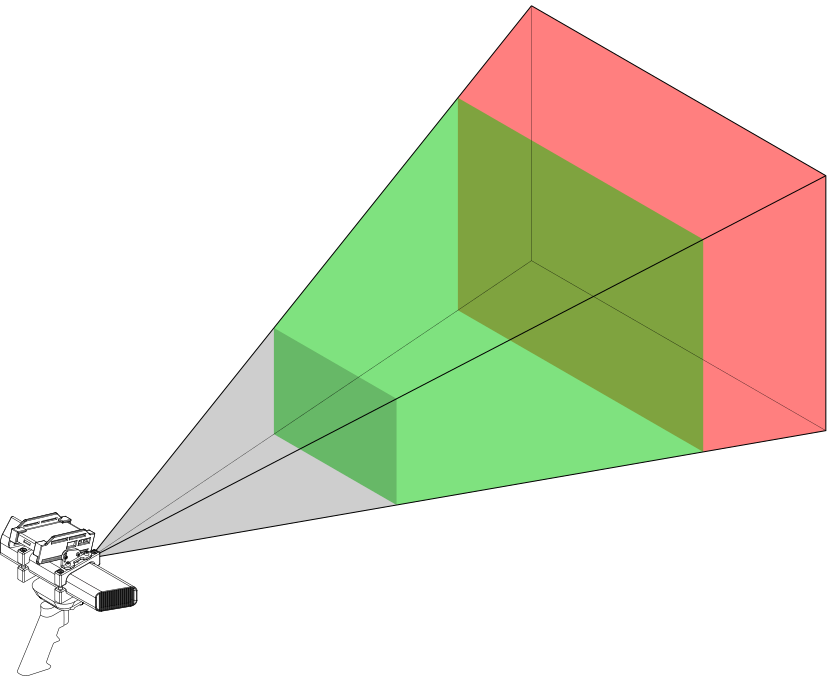
\includegraphics[scale=0.4]{interaktionsbereich}
		\caption{Parametrierbarer Interaktionsbereich}
		\label{fig.intfov}
	\end{center}
	%\vspace*{-18mm}
\end{figure}

\prever{
%\red[Bemaßung!\\]
}
Der minimale Abstand $z_\ind{{min}}$, in welchem Tiefeninformationen ausgewertet werden können, beträgt \SI{0,5}{\meter} und wird durch die Spezifikationen der Kinect definiert. Der maximale Interaktionsabstand $z_\ind{{int}}$ ist im Rahmen der Implementierung parametrierbar und kann damit anwendungsspezifisch definiert werden.\\

\nomenclature[l]{$z_\ind{{min}}$}{Minimal auflösbarer Tiefenwert der Kinect}
\nomenclature[l]{$z_\ind{{int}}$}{Maximaler Tiefenwert des Interaktionsbereichs}


Basierend auf den nach der Filterung verbleibenden Punkten wird eine Ebenendetektion nach \cite{Fischler1981} durchgeführt. Alle Punkte innerhalb eines definierten Abstandes werden daraufhin auf die ermittelte Ebene projiziert, wodurch eine zweidimensionale Abbildung erzeugt und Messwertrauschen geglättet wird. Außerhalb der Ebene liegende Punkte werden für die weiteren Schritte aus der Betrachtung entfernt. Dazu gehören deutliche Ausreißer innerhalb der detektierten Interaktionsstruktur sowie Artefakte in der Punktwolke.\\

Um eine gleichmäßige Objektstruktur zu erhalten wird anschließend eine Hüllkurve um die verbleibenden Punkte gelegt und die vorhandene Struktur mittels einer äquidistanten Verteilung von Punkten angenähert. Aus dieser Hüllkurve wird der geometrische Schwerpunkt (Basis) sowie der vom \kps{} am weitesten entfernte Punkt (Spitze) bestimmt. Der Verbindungsvektor zwischen Basis und Spitze bildet damit die Zeigerichtung des Anwenders ab. Der gesamte Ablauf zur Bestimmung der Zeigerichtung ist in \abb{fig.intdir} dargestellt.\\

\begin{figure}[!ht]
	\begin{center}
	\subfigure[Ausschnitt aus vollständiger Punktwolke]{
		\includegraphics[width=5cm]{interaction_01_02}
	}
	\hspace{5mm}
	\subfigure[Gefilterte Interaktionsstruktur abgebildet auf detektierte Ebene]{
		\includegraphics[width=5cm]{interaction_02_02}
	}
		\subfigure[Hüllkurve und geometrischer Schwerpunkt der Struktur]{
		\includegraphics[width=5cm]{interaction_03_02}
	}
	\hspace{5mm}
	\subfigure[Zeigerichtung definiert durch Verbindung zwischen Basis und Spitze]{
		\includegraphics[width=5cm]{interaction_04_02}
	}
	\caption{Filterung der Punktwolke zur Bestimmung der Zeigerichtung}
	\label{fig.intdir}
	\end{center}
	%\vspace*{-8mm}
\end{figure}

Um das Signal der ermittelten Linie zu glätten wird der gleitende Mittelwert der Punkte bestimmt. Auch die Differenz zwischen zwei Punkten aus aufeinander folgenden Messungen wird überwacht, um Sprünge in der Bewegung aufgrund von Fehldetektionen erkennen zu können. Aufgrund des implementierten Ansatzes wurde für die Kommunikation eine Nachrichtenstruktur definiert, welche die erkannte Linie abbildet. Das Modul \textit{Interaktion} stellt die ermittelte Linie über diese Nachricht zur Verfügung, so dass sie vom Softwaremodul \textit{Visualisierung} ausgewertet werden kann.\\

%Da die Kamera des Kinect Sensors auch von dem \mFovis verwendet wird besteht die Gefahr der Beeinflussung zwischen der Benutzereingabe und der lokalen Lokalisation. Um diese zu vermeiden sendet das \mInteraction Modul einen Befehl zum Pausieren der visuellen Odometrie sobald Punkte innerhalb des Interaktionsbereiches erkannt werden. Die visuelle Odometrie wird somit für die Dauer der Benutzerinteraktion unterbrochen. Sobald keine Punkte mehr innerhalb des Interaktionsbereiches detektiert werden, sendet das \mInteraction ein Signal zur Wiederaufnahme der visuellen Odometrie an das \mFovis .

Da die Kamera der Kinect auch zur Bestimmung der visuellen Odometrie verwendet wird, besteht die Möglichkeit, dass die lokale Lokalisation durch die Benutzereingabe beeinträchtigt wird. Um dies zu vermeiden wurde eine direkte Kommunikation zwischen den beteiligten Modulen implementiert. Die Berechnung der visuellen Odometrie wird dabei unterbrochen, sobald Punkte innerhalb des Interaktionsbereiches erkannt werden. Endet die Interaktion, kann die Ermittlung der visuellen Odometrie wieder aufgenommen werden. Im Falle kleiner Posenänderungen während der Benutzereingabe ist die Lokalisation in der Lage die Veränderungen zu erkennen und die Pose im Anschluss an die Benutzerinteraktion zu aktualisieren. Während der Interaktion sollte das Projektionsfeld jedoch ohnehin auf das ausgewählte Objekt ausgerichtet und eine starke Veränderung der Pose des \kps{s} vermieden werden.

\section{Erkennung von Befehlen}
Die Auswertung der auf Basis der Zeigebewegung ermittelten Linie erfolgt innerhalb des Moduls \textit{Visualisierung}. Die Detektion der Linie erfolgte im Koordinatensystem der Kamera $\ks{K}$, so dass diese für die Auswertung zunächst über $\tmat{M}{K}$ in das Koordinatensystem der Karte $\ks{M}$ transformiert wird.\\

Um zu bestimmen, auf welches Modellobjekt der Benutzer gezeigt hat, werden entlang der Linie alle Schnittpunkte mit den virtuellen Modelldaten bestimmt. Dazu wird die Visualisierungsumgebung VTK verwendet, welche die Ermittlung von Schnittpunkten zwischen den Modellobjekten und Linien als Funktion zur Verfügung stellt. Aus den Schnittpunkten kann somit ermittelt werden, welches Objekt der Benutzer ausgewählt hat. Um die Auswahl eines Objektes, analog einer \glqq Klick\grqq -Aktion, zu ermöglichen wurden zwei Verfahren implementiert. Die erste Implementierung erfolgt durch Überprüfung der Verweildauer des simulierten Zeigers auf dem Objekt. Überschreitet diese einen definierten Grenzwert wird dies als Auswahlbefehl gewertet und das Objekt in den Zustand \textit{aktiv} versetzt. Für das zweite Verfahren wurde die Software des Arduino um einen zusätzliche Schnittstelle erweitert. Durch die Anbindung eines Tasters wird die Möglichkeit einer echten \glqq Klick\grqq -Aktion zur Befehlseingabe realisiert. Durch Veränderung der Textur erhält der Anwender wie in \abb{fig.intintersect} dargestellt das visuelle Feedback, dass ein Objekt ausgewählt und in den neuen Status versetzt wurde.\\

\begin{figure}[!ht]
	\begin{center}
	\includegraphics[width=5cm]{model_selection_02}
	\caption{Auswahl eines Modellobjektes durch den Benutzer}
	\label{fig.intintersect}
	\end{center}
	%\vspace*{-8mm}
\end{figure}%
%
Innerhalb der Modellumgebung können nun temporäre Interaktionsobjekte wie in \abb{fig.intarrows} (a) dargestellt eingeblendet werden. Über das zuvor beschriebene Funktionsprinzip kann der Benutzer auch diese Objekte auswählen. Alle weiteren Modellobjekte werden während dieser Phase in den Status \textit{inaktiv} versetzt. Es ist somit immer nur ein Objekt der virtuellen Umgebung \textit{aktiv}, wodurch für den Anwender eine klare Zuordnung der Interaktionsobjekte möglich ist. Durch Auswahl der Interaktionsobjekte ist der Benutzer in der Lage das aktuell als \textit{aktiv} gewählte Objekt innerhalb der Modellumgebung zu modifizieren. \abb{fig.intarrows} (b) zeigt dies am Beispiel der Translation des Modellobjektes. Die Implementierung ermöglicht eine Modifikation der Objekte bezüglich aller sechs räumlichen Freiheitsgrade, so dass die Anzahl und Funktion der Interaktionsobjekte je nach Anwendungsfall spezifiziert werden kann.\\

\begin{figure}[!ht]
	\begin{center}
	\subfigure[Auswahl eines temporären Interaktionsobjektes]{
		\includegraphics[width=5cm]{model_selection_04}
	}
	\hspace{5mm}
	\subfigure[Bewegtes Modellobjekt mit aktualisierten Interaktionsobjekten]{
		\includegraphics[width=5cm]{model_selection_05}
	}
	\caption{Modifikation der Position des Modellobjektes durch Auswahl eines Interaktionsobjektes}
	\label{fig.intarrows}
	\end{center}
	%\vspace*{-8mm}
\end{figure}

Durch die Erkennung der Benutzereingabe können somit Objekte der Modellumgebung ausgewählt und bezüglich ihrer Pose modifiziert werden. Die Integration der Interaktion in die Visualisierung ermöglicht die direkte Modifikation der zugrunde liegenden Modelldaten. Das aktualisierte Modell kann abschließend gesichert werden, wodurch eine Rückführung in den virtuellen Modellierungs- und Planungsprozess erreicht wird.

\prever{
%\red[Intersection sollte auch mit Modellumgebung möglich sein, damit der Pointer realistisch abgebildet wird!? Vielleicht Modell (obj) der Karte mit schwarzer Textur?]
}
    \chapter{Datenkopplung}
\red[TODO:\\
Kapitel entfernen? Hat eigentlich keine Relevanz, wenn Datenkopplung schon in 4 Beschrieben ist\\
]
\section{Modifikation der Modelldaten}
Siehe Kapitel \ref{chap:modell}. An welcher Stelle besser geeignet?

\section{Sichern des aktualisierten Modells}
Siehe Kapitel \ref{chap:modell}. An welcher Stelle besser geeignet?

    \chapter{Auswertung und Ergebnisse}
\label{chap.results}
\red[TODO:\\
PGFPlots einfügen\\
Daten aufbereiten\\
Ergebnisse vergleichen/auswerten\\
]

Um die Funktionalität des \kps{s} bewerten und verschiedene Anwendungsfälle vergleichen zu können wird eine experimentelle Evaluation durchgeführt. Diese soll besonders dazu dienen Fehlereinflüsse der einzelnen Schritte zwischen der Lokalisation des Systems und der Darstellung der visuelle Zusatzinformationen zu quantifizieren. Zunächst erfolgt eine Betrachtung der Lokalisationsgenauigkeit. Dazu wird die globale Lokalisation auf Basis der zwei in \kapitel{chap.globloc} beschriebenen Modelle durchgeführt. Anschließend erfolgt die Bestimmung der Fehlereinflüsse der visuellen Odometrie und der inertialen Messeinheit auf die lokale Positionsbestimmung. Abschließend wird eine gesonderte Betrachtung der Transformation zwischen Kamera und Projektor durchgeführt.\\
Als Bewertungsreferenz (Ground Truth) der Lokalisation werden die in \abb{fig.armarker} gezeigten Markerfelder verwendet.

\begin{figure}[!ht]
	\begin{center}
		\includegraphics[scale=1.0]{spacer}
		\caption{AR Markerfelder}
		\label{fig.armarker}
	\end{center}
	%\vspace*{-8mm}
\end{figure}

Durch Erfassung in Kamerabildern können Orientierung und Ursprung der Felder bestimmt werden \red[näher erläuteren?]. Je Feld werden vier Marker aufgebracht um die Robustheit der Detektion zu erhöhen. Die jeweilige Positionierung der Felder ist abhängig von der jewiligen Untersuchung und wird innerhalb der folgenden Abschnitte detaillierter beschrieben. 

\section{Globale Lokalisation}
Die globale Lokalisation bildet die Basis der Positionsbestimmung. Dabei ist besonders eine approximative Bestimmung der Systempose von Bedeutung. Die Bestimmung einer möglichst exakten Annäherung der Pose ist zwar prinzipiell ebenso Ziel der globalen Lokalisation, kann jedoch bei korrekter initialer Approximation auch durch anschließende Optimierungsschritte erreicht werden. Im Falle einer fehlerhaften initialen Lokalisation kann trotz einer lokalen Optimierung nicht von einer Verringerung der Abweichung zur wahren Pose ausgegangen werden. Als zusätzliches Bewertungskriterium der globale Lokalisation wird deshalb im Folgenden neben der Abweichung zur realen Pose auch die Erfolgswahrscheinlichkeit der Approximation erfasst.\\

Um die wahre Pose des \kps{s} zu bestimmen wird das Markerfeld innerhalb der realen Umgebung auf einer glatten Fläche befestigt. Der Abgleich zwischen der daraus bestimmten Pose und der durch die Lokalisation ermittelten Pose ist dabei nur möglich, wenn die Pose des Markerfeldes auch in der Modellumgebung bekannt ist. Dies kann entweder durch Anbringung der Markerfelder vor der Kartierung oder durch Definition der Markerpose anhand eindeutiger Landmarken der Umgebung erreicht werden.\\

Die Bestimmung der Referenzpose kann nun durch Erfassung des Markerfeldes mit der Kamera des Systems erfolgen. Dazu wird das \kps{} in einer Pose fixiert und die Transformation zwischen dem Markerfeld und dem \kps{} bestimmt. Durch die vorhandene Verknüpfung zwischen der realen und der Modellumgebung ist die Transformation zwischen den Koordinatensystemen der Karte und des Markerfeldes beschrieben\red[ Bild?]. Es lässt sich somit die Transformation zwischen \kps{} und Karte bestimmen:

\begin{equation}
\tmat{M}{K} = \tmat{M}{AR}\tmat{AR}{K}
\end{equation}

Auch die globale Lokalisation wird durchgeführt während sich das \kps{} in der fixierten Pose befindet. Die so ermittelte Pose kann nun mit der Referenzposition verglichen werden. Im folgenden werden die Ergebnisse in Abhängigkeit des verwendeten Modells beschrieben. Die Fehlerwerte wurden dabei für alle Untersuchungen als Quadratischer Mittelwert über die Messungen bestimmt:

\begin{equation}
QMW = \sqrt{\frac{1}{n}\sum_{i=1}^nr_i^2}
\end{equation}

Aufgrund der Programmstruktur ist die Vorgabe eines Bereiches zur Verteilung der Partikel bezüglich der \red[z-Koordinate] der Karte erforderlich. Da das handgeführte \kps{} zu Beginn der Anwendung leicht in einer definierten Höhe bewegt werden kann, wurde dieser Grenzbereich mit einer Toleranz von $\pm$ \SI{0,1}{\meter} zur tatsächlichen Pose definiert.\\
\red[\abb{fig.error_glob_trans} zeigt den Vergleich der durch die beiden Modelle erzielten Fehlerwerte.\\]

\begin{tikzpicture}
\begin{axis}[
	ybar,
	ymax=0.4,
	ymin=0,
	bar width=30pt,
	enlarge x limits=0.4,
	legend style={at={(0.5,-0.15)},
	anchor=north,legend columns=-1},
	ylabel={Positionsfehler \lbrack m\rbrack},
%	symbolic x coords={\Delta,y,z},
	xticklabels={$\Delta X$, $\Delta Y$, $\Delta Z$},
	xtick=data,
	every node near coord/.style={/pgf/number format/fixed, anchor=west},
	nodes near coords,
	nodes near coords align={vertical},
	width=14cm,
	height=8cm,
	grid=major,
    	grid style={dotted,lightgray!80!white},
    	scaled y ticks = false,
]
\addplot[
	every node near coord/.append style={xshift=-1.1cm},
	nodes near coords=\raisebox{0.7cm}{\pgfmathprintnumber\pgfplotspointmeta},
	color=red,
	fill=red!30!white
] coordinates {(-1,0.3105647208) (0,0.3388888731) (1,0.0473358078)};
\addplot[
	every node near coord/.append style={xshift=0.0cm},
	nodes near coords=\raisebox{0.7cm}{\pgfmathprintnumber\pgfplotspointmeta},
	color=blue,
	fill=blue!30!white
] coordinates {(-1,0.1315834135) (0,0.1248760865) (1,0.0209899568)};
\legend{Raycasting,Endpoint}
\end{axis}
\label{fig.error_glob_trans}
\end{tikzpicture}

\red[Winkelfehler Vergleich:\\]

\begin{tikzpicture}
\begin{axis}[
	ybar,
	ymax=10,
	ymin=0,
	bar width=30pt,
%	enlarge y limits={0.4,upper},
	enlarge x limits=0.4,
	legend style={at={(0.5,-0.15)},
	anchor=north,legend columns=-1},
	ylabel={Winkelfehler \lbrack °\rbrack},
%	symbolic x coords={\Delta,y,z},
	xticklabels={$\Delta X$, $\Delta Y$, $\Delta Z$},
	xtick=data,
	every node near coord/.style={/pgf/number format/fixed, anchor=west},
	nodes near coords,
	nodes near coords align={vertical},
	width=14cm,
	height=8cm,
	grid=major,
    	grid style={dotted,lightgray!80!white},
    	scaled y ticks = false,
]
\addplot[
	every node near coord/.append style={xshift=-1.1cm},
	nodes near coords=\raisebox{0.7cm}{\pgfmathprintnumber\pgfplotspointmeta},
	color=red,
	fill=red!30!white
] coordinates {(-1,2.4445637073) (0,0.9069805767) (1,8.4545773848)};
\addplot[
	every node near coord/.append style={xshift=0.0cm},
	nodes near coords=\raisebox{0.7cm}{\pgfmathprintnumber\pgfplotspointmeta},
	color=blue,
	fill=blue!30!white
] coordinates {(-1,3.1694824628) (0,1.6633422885) (1,4.2398218425)};
\legend{Raycasting,Endpoint}
\end{axis}
\label{fig.error_glob_trans}
\end{tikzpicture}

Um die erfolgreiche Approximation der Pose zu bewerten wird wie in \abb{fig.loclimits} dargestellt ein Grenzraum um die wahre Position definiert. Darüber hinaus werden ebenfalls Grenzbereiche für die maximal zulässigen Winkelfehler festgelegt. Die zugehörigen Werte sind in \tab{thresh_glob} aufgeführt.\\

\begin{figure}[!ht]
	\begin{center}
		\includegraphics[scale=1.0]{spacer}
		\caption{Grenzbereich der Lokalisation}
		\label{fig.loclimits}
	\end{center}
	%\vspace*{-8mm}
\end{figure}

\begin{table}[ht]
	\centering
	\caption{Grenzwerte zur Bestimmung der erfolgreichen Approximation}\label{tab.TechSpecYouBotBase}
	\vspace*{-3mm}
	\begin{tabular}[ht]{|l|r|}\hline
		\rowcolor{Snow2}
		Dimension		& Grenzwert 					\\ \hline
		X				& \SI{1}{\milli\meter}		\\ \hline		
		Y				& \SI{1}{\milli\meter}		\\ \hline
		Z				& \SI{1}{\milli\meter}		\\ \hline
		Yaw				& \SI{1}{\milli\meter}		\\ \hline
		Pitch			& \SI{1}{\milli\meter}		\\ \hline
		Roll 			& \SI{1}{\milli\meter}		\\ \hline		
		\hline
	\end{tabular} 
	\vspace*{-3mm}
\end{table}

\red[Quadratischer Mittelwert QMW statt Root Mean Square RMS überall aktualisieren]

\subsection{Raycasting-Modell}

\subsection{Endpoint-Modell}

\red[Relokalisation bei globaler Lokalisation beschreiben]

\section{Lokale Lokalisation}%Tracking/Kontinuierliche Lokalisation}
Die Genauigkeit der lokalen Lokalisations wird gesondert von der durch die globale Lokalisation bestimmten Pose betrachtet. Dazu wird ebenfalls das für die Untersuchung der globalen Lokalisation verwendete Markerfeld genutzt. Die wahre Pose des Systems kann so bestimmt und als Initialisierung der Lokalisation verwendet werden.\\
Die Bewertung der kontinuierlichen Lokalisation erfolgt gesondert für translatorische und rotatorische Bewegungen. Alle Messungen werden dabei separat durchgeführt um eine Beeinflussung der Bewegungen untereinander zu verhindern. Translatorisch werden dabei die Bewegung parallel (x-Achse der Kamera) und orthogonal (z-Achse der Kamera) zu einer Ebene betrachtet. Die parallele Bewegung wird dabei lediglich entlang einer Achse durchgeführt, da diese für beide Achsen parallel zur Ebene äquivalent ist und nur durch die Orientierung der Koordinatensysteme definiert wird. Ähnliches gilt für die Untersuchung der Lokalisationsgenauigkeit bei rotatorischen Bewegungen des Systems, da der Algorithmus der visuellen Odometrie nicht zwischen den Rotationsachsen der Kamera unterscheidet. Die Lokalisation während der Rotationsbewegungen wird zunächst allein auf Basis der visuellen Odometrie und anschließend allein auf Basis der inertialen Messeinheit durchgeführt. Abschließend erfolgt eine Bewertung der Lokalisation nach Fusion der beiden Sensorsysteme mittels des Erweiterten Kalman Filters.

\subsection{Translation X}

\subsection{Translation Z}

\subsection{Rotation Yaw}

\subsection{Rotation Pitch FOVIS}

\subsection{Rotation Roll FOVIS}

\subsection{Rotation Pitch IMU}

\subsection{Rotation Roll IMU}

\subsection{Rotation Pitch KALMAN}

\subsection{Rotation Roll KALMAN}

%Die globale Lokalisation wird anhand des Boards korrigiert um eine definierte Ausgangslage zu erhalten. Anschließend erfolgt eine Bewegung des Kamera-Projektor Systems entlang der verschiedenen Raumrichtungen und eine Rotation um die jeweiligen Winkel. Alle Messungen werden separat durchgeführt um eine Beeinflussung der Parameter untereinander zu verhindern. Die Bewegung erfolgt so, dass eine Rückkehr zur Ausgangslage stattfindet um eine Bestimmung der Positionsabweichung im Anschluss an die Bewegung durch erneute Detektion des Boards zu ermöglichen. Es ist darauf hinzuweisen, dass aufgrund der getrennten Betrachtung die Validierung zum einen für die visuelle Odometrie (x,y,z,yaw) und zum anderen für die Messdaten der IMU erfolgt (roll, pitch).

\section{Projektionsgenauigkeit}
Die Genauigkeit der Projektion virtueller Modelldaten wird unter Verwendung einer externen Kamera durchgeführt. Diese wird zunächst analog zum Vorgehen für die RGB-Kamera des Kinect Sensors kalibriert (siehe \kapitel{chap.calib}). Dadurch wird eine objektive Betrachtung der Projektionsgenauigkeit ermöglicht, da diese maßgeblich von der Kalibrierung des \kps{s} abhängt. Für die Untersuchung wird ein Markerfeld auf einer ebenen Unterlage fixiert und im Sichtfeld der RGB-Kamera des Kinect Sensors platziert. Durch die Erfassung des Markerfeldes und der daraus bestimmten Transformation kann die Position des \kps{s} relativ zum Markerfeld bestimmt werden.\red[ Markerfelder abbilden? Erstes Oben schon, zweites hier?]\\

Die bekannte Transformation zwischen Kamera- und Projektorkoordinaten ermöglicht nun die Zuordnung der detektierten 3D-Koordinaten des Markerfeldes zu den 2D-Koordinaten des Projektorbildes. Um die Projektionsgenauigkeit zu überprüfen wird nun mittels des Projektors ein weiteres Markerfeld projiziert, welches bezogen auf die Projektorkoordinaten deckungsgleich mit dem realen Markerfeld ist. \red[\abb{fig.arprojected}]\\

\begin{figure}[!ht]
	\begin{center}
		\includegraphics[scale=0.5]{board_eval_cropped}
		\caption{AR Marker real und projiziert}
		\label{fig.arprojected}
	\end{center}
	%\vspace*{-8mm}
\end{figure}

Die externe Kamera wird nun eingesetzt, um beide Markerfelder gleichzeitig zu erfassen und die Abweichungen zwischen den Feldern bezüglich Position und Orientierung zu bestimmen. Dabei werden die Positionierungen sowohl des \kps{s} als auch der externen Kamera während der Untersuchungen variiert. \red[Die Bestimmung der Fehlerwerte erfolgt erneut über Berechnung des QMW.\\
Die Ergebnisse der $n=6$ Messreihen sind in \tab{projection} zusammengefasst.]\\
Der Box-Whisker-Plot in \abb{fig.boxplot_proj} zeigt die Verteilung der translatorischen Fehlerwerte entlang der Raumachsen.\\

\begin{figure}
\begin{center}
\begin{tikzpicture}[trim axis left, trim axis right]
  \begin{axis}[
    	ytick={-30,-20,...,30},
    		minor y tick num=3,
    		ymax=35,
    		ymin=-35,
    		ylabel=Y-Achse \lbrack mm\rbrack,
    		xtick={1,...,3},
    		x tick label style={align=center},
    		xticklabels={$\Delta X$,$\Delta Y$,$\Delta Z$},
    		boxplot/draw direction=y,
    		width=14cm,
    		height=8cm,
    		grid=major,
    		grid style={dotted,lightgray!80!white},
    ]
    \addplot+[color=red,mark=x,
    		boxplot prepared={
      		lower whisker=-7.2937458753,
      		lower quartile=-2.2697057575,
      		median=-0.5078930408,
      		upper quartile=2.5787912309,
      		upper whisker=5.2836090326,
      		box extend=0.5,
    		},
    ] coordinates {};
    %table[row sep=\\,y index=0] {0.0\\}; %Ausreisser
    \addplot+[color=Green,mark=x,
    		boxplot prepared={
      		lower whisker=-5.6481547653,
      		lower quartile=0.8273310959,
      		median=2.7935747058,
      		upper quartile=6.1452584341,
      		upper whisker=6.959207356,
			box extend=0.5,
		},
    ] coordinates {};
    %table[row sep=\\,y index=0] {0.0\\}; %Ausreisser
    \addplot+[color=blue,mark=x,
    		boxplot prepared={
      		lower whisker=-30.851304531,
      		lower quartile=-12.757569552,
      		median=5.149245262,
      		upper quartile=11.0025405888,
      		upper whisker=22.670924664,
%      		lower whisker=-9.7615455743,
%      		lower quartile=-4.0365747411,
%      		median=1.6292533837,
%      		upper quartile=3.4812726082,
%      		upper whisker=7.173222257,
			box extend=0.5,
		},
    ] coordinates {};
    %table[row sep=\\,y index=0] {0.0\\}; %Ausreisser
  \end{axis}
\end{tikzpicture}
\caption{Box-Whisker-Plot}
\label{fig.boxplot_proj}
\end{center}
\vspace{-3mm}
\end{figure}

\red[Öffnungswinkel $\sim$ 30°, dadurch Faktor 16/9 für Fehlerwerte in z-Richtung. Sogar (16/9)² für Detektion+Projektion? Dann würden sich die Werte auf jeden Fall stark annähern]

\red[Nennen, dass Boxplot ganze Messreihe abbildet! Oder umwandeln zu 5/95 Perzentil?\\]

\begin{table}[ht]
	\centering
	\caption{Technische Daten der youBot Plattform}\label{tab.TechSpecYouBotBase}
	\vspace*{-3mm}
	\begin{tabular}[ht]{|l|c|r|}\hline
		\rowcolor{Snow2}
		Bezeichnung						& Formelzeichen	& \\ \hline
		Gesamtlänge 					&			& \SI{530}{\milli\meter}				\\ \hline
		Gesamtbreite 					&  		& \SI{350}{\milli\meter}				\\ \hline
		Höhe									&  		& \SI{106}{\milli\meter}				\\ \hline
		Radstand							& $l$	& \SI{470}{\milli\meter}				\\
		\hline
	\end{tabular} 
	\vspace*{-3mm}
\end{table}


%Überprüfung der Genauigkeit mit Hilfe externer Kamera. Externe Kamera wird kalibriert um objektive Betrachtung der Projektionsgenauigkeit zu ermöglichen. Kamera Projektor System ist bereits kalibriert. Verwendung von 2 QR Boards. Eins wird auf ebene Unterlage aufgeklebt, das andere wird vom Projektor projiziert. Zunächst wird das aufgeklebte Board durch die Kamera des Kamera Projektor Systems erkannt um daraus die Transformation zu berechnen, welche im Programm verwendet wird um die Projektorsicht zu erzeugen. Das projizierte Board wird anschließend mit der externen Kamera erfasst genauso wie das aufgeklebt. Es wird jeweils die Transformation zur Kamera berechnet um daraus die Differenz der beiden Boards bezüglich Position und Lage zu bestimmen.

\section{Benutzerinteraktion}

\begin{figure}[!ht]
\vspace{3mm}
\begin{center}
\begin{tikzpicture}[trim axis left, trim axis right]
	\begin{axis}[
		xlabel=X,
		ylabel=Y,
		xtick={1,...,13},
		ymin=0,
		ytick={0,10,...,100},
		legend style={
			at={(1,0.5)},
			xshift=0.2cm,
			anchor=north west,
			nodes=right,
			draw=none
		},
		grid=major,
   		grid style={dotted,lightgray!80!white},
		%axis lines=left
		width=14cm,
		height=7cm,
	]
	\addplot[color=red] coordinates{
		(1,24.6718)
		(2,43.7092)
		(3,54.14785132)
		(4,63.1821339)
		(5,70.60866985)
		(6,76.45681086)
		(7,81.7263871)
		(8,86.97406846)
		(9,90.86684525)
		(10,93.72329021)
		(11,96.11621437)
		(12,98.25885879)
		(13,100)		
	};
	\addplot[color=blue] coordinates{
		(1,26.42529337)
		(2,51.19458535)
		(3,63.64859236)
		(4,72.13773673)
		(5,78.8676646)
		(6,83.94694845)
		(7,88.06842906)
		(8,91.7882484)
		(9,94.19470806)
		(10,96.53607266)
		(11,98.45170481)
		(12,100)
		
	};
	\legend{Testa,Testb}
	\end{axis}
\end{tikzpicture}
\end{center}
\vspace{-3mm}
\caption{test1}
\label{fig.test1}
\vspace{3mm}
\end{figure}

\begin{figure}[ht]
\centering
\begin{tikzpicture}
\begin{axis}[
xlabel={Zeit},
ylabel={Position},
ymin=0,
ymax=6,
width=100mm,
height=80mm,
ytick={0,1,...,5},
legend style={at={(1,1)},	anchor=north east, xshift=-1mm,	yshift=-1mm}
]
\pgfplotstableread{plot/test.txt}\datatable
\addplot[color=red,mark=square*] table[x index=0,y index=1] from \datatable;
%\addplot[no markers] table[x index=0,y index=3] from \datatable;
%\addplot[no markers] table[y = Leistung] {plot/test.txt}  ;
\legend{test}
\end{axis}
\end{tikzpicture}
\caption{test2}
\label{fig.test2}
\end{figure}

\begin{figure}
\begin{center}
\begin{tikzpicture}[trim axis left, trim axis right]
  \begin{axis}[
    	ytick={0,0.1,...,1.1},
    		minor y tick num=5,
    		ymax=1.1,
    		ylabel=Y-Achse,
    		xtick={1,...,4},
    		x tick label style={align=center},
    		xticklabels={A, B},
    		boxplot/draw direction=y,
    		width=8cm,
    		height=8cm,
    		thick,
    ]
%    \addplot+[color=red,mark=x,
%    		boxplot prepared={
%      		lower whisker=,
%      		lower quartile=,
%      		median=,
%      		upper quartile=,
%      		upper whisker=
%    		},
%    ] %coordinates {};
%    table[row sep=\\,y index=0] {0.7054\\ 0.9773\\  0.9763\\ 0.9698\\ 0.7118\\ 0.6919\\ 0.9727\\ 0.7006\\ 0.974\\ 0.7077\\}; %Ausreisser
    \addplot+[color=Green,mark=x,
    		boxplot prepared={
      		median=0.3036,
      		upper quartile=0.34925,
      		lower quartile=0.2674,
      		upper whisker=0.5597,
      		lower whisker=0.18718
		},
    ] %coordinates {};
    table[row sep=\\,y index=0] {0.6045\\ 0.1818\\ 0.5826\\ 0.5688\\ 0.1814\\ 0.1825\\ 0.5750\\ 0.1783\\ 0.6312\\ 0.1793\\}; %Ausreisser
  \end{axis}
\end{tikzpicture}
\caption{Box-Whisker-Plot}
\label{fig.error_boxplot}
\end{center}
\vspace{-3mm}
\end{figure}
    \chapter{Zusammenfassung und Ausblick}
\label{chap:zusammenfassung}
\red[TODO:\\
Entwickeltes System kurz zusammenfassen, beginnend damit warum es erstellt wurde!\\
Ergebnisse und Fazit daraus kurz zusammenfassen\\
Ausblick geben auf erweiterungen des Systems - Um die Einsschränkungen zu beheben - Um das System zu erweitern/verbessern\\
Ausblick geben auf mögliche Anwendungsfälle/-gebiete\\
Limitierungen in Ausblick aufnehmen\\
Bimber - Embedded Entertainment with Smart Projectors -> für Ausblick/Limitierungen bzgl. der Projektionsuntergründe
auch Park - Kontrast erhöhung
auch Wang - Relighting\\
Bimber - Multi-Projector Techniques for Real Time... -> Architectural Projection\\
Anpassung der Varianz im Sensormodell in Abhängigkeit der Entfernung\\
Ground Truth über externes Lokalisationssystem bestimmen\\
]

\kps{} erstellt zur Darstellung visueller Zusatzinformationen;\\
Selbstlokalisation durch Partikelfilter verwendet;\\
Tracking basierend auf visueller Odometrie verwendet;\\
Robustheit durch IMU und Kalman-Filter gesteigert;\\
Projektion von Modelldaten, Projektor als inverse Kamera, die Modellszene betrachtet, eigentlich nicht mehr direkt invers dann;\\
Gesamtsystem kalibriert;\\
Grafische Benutzeroberfläche erstellt, welche die Funktionen zugänglich macht, ist aber für Anwendung nicht unbedingt erforderlich, dann muss vorher die Welt definiert werden;\\
Buttons integriert;\\
Anbindung an ROS ermöglicht Austausch verschiedener Module;

System ermöglicht Lokalisation und Darstellung visueller Zusatzinformationen;\\
Anwendung unterliegt ein paar Einschränkungen, die jedoch im geplanten Anwendungsszenario keine Probleme machen sollten; Unter Berücksichtigung der Empfehlungen aus dem vorhergehenden Kapitel;\\

Erweiterungen:\\
Kinect V2;\\
Kompass zur Lagebestimmung yaw -> deutliche Reduzierung der Partikelanzahl möglich;\\
Gestenerkennung -> Kinect V2 gut, da bessere Auflösung;\\
Projektion auf beliebige Oberflächen -> Arbeiten siehe Stand der Technik\\

    %\nocite{*}                             % alle Literaturquellen einbinden, sonst werden nur die zitierten
                                            % Quellen im Literaturverzeichnis angezeigt (ist Geschmackssache).
                                            % eher nicht verwenden, au�er man hat einen guten Grund
                                            
	%% --- Literaturverzeichnis
    \bibliographystyle{alphadin}            % Darstellung nach DIN, mit Name und Jahr z.B. [Sch06]
    \bibliography{masterbib}                % Literaturverzeichnis einbinden                                            
                                            
                                            
    \appendix                               % Anhang starten, jedes weitere Kapitel bekommt jetzt einen Buchstaben
    \chapter*{Anhang}                       % Anhang als Chapter
    \thispagestyle{empty}                   % keine Kopfzeile, Seitenzahl u.a., leere Seite mit �berschrift Anhang
    \setcounter{chapter}{1}                 % Chapter Counter auf 1 = im Anhang A
    \setcounter{equation}{0}                % Equation Counter nullen
    \addstarredchapter{Anhang}              % Minitoc mitteilen, dass neues Chapter
    \newpage                                
    \ihead{\normalfont Anhang}              % Kopfzeile auf Anhang setzen
    
    \minitoc                                % Anhangsverzeichnis plotten
    %% --- Ab hier der Anhang einf�gen

    \section{1}
\label{app_1}

\clearpage{}

\section{2}
\label{app_2}

\clearpage{}            % Anhang
    %\include{anhang_fehlerfortpflanzung}
		%\include{anhang_mgcEinstellungen}
		%\include{anhang_trafos}
		%\include{anhang_befestigen}
		%\include{anhang_datenblaetter}
  

    %% --- Anhang zu Ende
    \ihead{\normalfont\headmark}            % kolumnentitel innen
 
    

\end{spacing}
\end{document}                              % fertig!